\PassOptionsToPackage{usenames,fixpdftex,dvipsnames,svgnames,x11names}{xcolor}
\PassOptionsToPackage{hyphens}{url}
\PassOptionsToPackage{font=small,labelfont=bf,labelsep=period}{caption}

\documentclass[
  oneside,
  openany,
  numbers=noendperiod,
  parskip=half,
  bibliography=totoc
]{scrbook}

% Page layout
\usepackage[
  a4paper,
  left=23mm,
  top=27.4mm,
  bottom=27.4mm,
  %headsep=2\baselineskip,
  textwidth=107mm,
  marginparsep=8mm,
  marginparwidth=49mm,
  %textheight=49\baselineskip,
  %headheight=\baselineskip
]{geometry}
%\usepackage{showframe}
\usepackage{multicol}

% Margin paragraph
\usepackage{sidenotes}
\usepackage{marginfix}
%\usepackage{morefloats} % More than 18 floats

% Headers and footers
\usepackage[
  automark,
  headsepline=false,
  headwidth=textwithmarginpar,
  footwidth=head
]{scrlayer-scrpage}

\clearpairofpagestyles
\rofoot[\pagemark]{\pagemark}
\lohead{\headmark}

% Title page
\title{eulerr: Area-Proportional Euler Diagrams with Ellipses}
\author{Johan larsson}
\date{\today}

\renewcommand{\maketitle}{%
  \cleardoublepage
  \begin{fullwidth}
  \centering
  \vspace*{3cm}
  
\includegraphics[width=0.3\textwidth]{LundUniversity_C2line_BLACK}\par\vspace{1cm}
  \vspace{0.5cm}
  {\scshape\Large Bachelor Thesis \par}
  {\Huge\bfseries eulerr: Area-Proportional Euler Diagrams with Ellipses \par}
  \vspace{2cm}
  {\huge\itshape Johan Larsson \par}
  \vspace{2cm}
  {\Large{\itshape supervised by}\par Peter Gustafsson}
  \vfill
  {\large \today\par}
  \end{fullwidth}
  \thispagestyle{empty}
}

% Graphics
\usepackage[font=footnotesize]{subcaption}
\usepackage{graphicx}
\setkeys{Gin}{width=\linewidth,totalheight=\textheight,keepaspectratio}
\graphicspath{{graphics/}}
%\captionsetup[sub]{font = footnotesize}

\usepackage{booktabs}
%\usepackage[header,page]{appendix}

% Text justification and parskip
\usepackage[document]{ragged2e}
%\setlength{\RaggedRightParindent}{\parindent}

% Lists
\usepackage[shortlabels]{enumitem}
%\setlist{listparindent=\parindent, parsep=0pt plus 1pt}

% Algorithms
\usepackage[vlined]{algorithm2e}

% Babel
%\usepackage[swedish]{babel}

% Bibliography
\usepackage[square,numbers,sort&compress]{natbib}
\usepackage{etoolbox}
%\usepackage{relsize}
\patchcmd{\thebibliography}
  {\list}
  {\begin{multicols}{2}\small\list}
  {}
  {}
\appto{\endthebibliography}{\end{multicols}}

% Floats
\DeclareCaptionType[fileext=alg,name=Algorithm]{alg}

% Extended verbatim environments
\usepackage{fancyvrb}
\fvset{fontsize=\small}% default font size for fancy-verbatim environments

% Provide fullwidth environment
\newlength{\overhang}
\setlength{\overhang}{\marginparwidth}
\addtolength{\overhang}{\marginparsep}
\makeatother

\newenvironment{fullwidth}{
  \begin{addmargin*}[0em]{-\overhang}
  }{
  \end{addmargin*}
}

% Fonts
\usepackage[utf8]{inputenc}
\usepackage[T1]{fontenc}
\usepackage[lining]{libertine}
\usepackage{textcomp}
\usepackage[varqu,varl,scaled=0.93]{inconsolata}
\usepackage{mathtools}
\usepackage{amsthm}
\usepackage[libertine,vvarbb,libaltvw,liby]{newtxmath}
\usepackage[scr=rsfso]{mathalfa}
\usepackage{bm}
\useosf
\usepackage{microtype}

\newcommand{\proglang}[1]{\textsf{#1}}
\newcommand{\pkg}[1]{{\fontseries{b}\selectfont #1}}
\newcommand{\code}[1]{\texttt{#1}}

% Custom operators
\DeclareMathOperator{\E}{E}
\DeclareMathOperator{\Pois}{Pois}
\DeclareMathOperator{\B}{Bin}
\DeclareMathOperator{\V}{Var}
\DeclareMathOperator{\Exp}{Exp}

% Caption styles (caption package is loaded with sidenotes)
\DeclareCaptionStyle{sidecaption}{labelfont=bf,labelsep=period,font=small}
\DeclareCaptionStyle{marginfigure}{labelfont=bf,labelsep=period,font=small}
\DeclareCaptionStyle{margintable}{labelfont=bf,labelsep=period,font=small}
\DeclareCaptionStyle{widefigure}{labelfont=bf,labelsep=period,font=small}
\DeclareCaptionStyle{widetable}{labelfont=bf,labelsep=period,font=small}

% Cross-referencing and colors
\usepackage{hyperref}
\usepackage[noabbrev,capitalize,nameinlink]{cleveref}
\usepackage{xcolor}
\hypersetup{linkcolor=SteelBlue4,
            citecolor=SteelBlue4,
            urlcolor=SteelBlue4,
            colorlinks=true,
            breaklinks=true}

% Theorems
\newtheorem{mydef}{Definition}[chapter]

% Custom title page


% Change fontsize in sidenotes
\makeatletter
\ExplSyntaxOn
\RenewDocumentCommand \sidenotetext { o o +m }
{
  \IfNoValueOrEmptyTF{#1}
    {
      \@sidenotes@placemarginal{#2}{\textsuperscript{\thesidenote}{}\small~#3}
  \refstepcounter{sidenote}
}
    {\@sidenotes@placemarginal{#2}{\textsuperscript{#1}\small~#3}}
}
\ExplSyntaxOff
\makeatother

% Fix vdots and ddots for smallmatrix
\newcommand{\svdots}{\raisebox{3pt}{$\scalebox{.75}{\vdots}$}}
\newcommand{\sddots}{\raisebox{3pt}{$\scalebox{.75}{$\ddots$}$}}

% Rotate text 90 degrees (for table)
\newcommand*\rot{\rotatebox{90}}

% Libertine in tabular
\makeatletter
\AtBeginDocument{\def\libertine@figurealign{}\libertineOsF}
\newcommand\libertineTabular{\def\libertine@figurealign{T}\libertineLF}
\makeatother

\begin{document}



\frontmatter

\maketitle

\begin{addmargin*}[0.5\overhang]{-0.5\overhang}
{\hypersetup{linkcolor=black}
\tableofcontents
}
\end{addmargin*}
\mainmatter

\chapter{Background}\label{sec:background}

The visual display of data represents an intuitive form of data presentation.
Data visualizations work on multiple dimensions and possess the
potential to convey intricate relationships that single statistics or tables
never can.

Such visualizations, however, are only effective if their aesthetics convey
relationships. Consider, for instance, a disc with a radius of 2~cm labelled
\emph{Men}\marginpar{%
\begin{knitrout}\small
\definecolor{shadecolor}{rgb}{0.969, 0.969, 0.969}\color{fgcolor}

{\centering \includegraphics[width=\maxwidth]{figure/graphics-men-1} 

}



\end{knitrout}
}---it says nothing by itself; yet if we juxtapose it with a 1~cm-radius disc
labelled \emph{Children}\marginpar{%
\begin{knitrout}\small
\definecolor{shadecolor}{rgb}{0.969, 0.969, 0.969}\color{fgcolor}

{\centering \includegraphics[width=\maxwidth]{figure/graphics-children-1} 

}



\end{knitrout}
}, the graphic starts to become informative: it now displays the relation
between two quantities. Now, if we intersect the two
discs, so as to produce an overlap, we have successfully visualized the
relative proportions of men and men, as well as their intersection. The diagram
we have constructed is a \emph{Euler diagram}~(\cref{fig:children-men}).

\begin{marginfigure}
\begin{knitrout}\small
\definecolor{shadecolor}{rgb}{0.969, 0.969, 0.969}\color{fgcolor}

{\centering \includegraphics[width=\maxwidth]{figure/graphics-childrenMen-1} 

}



\end{knitrout}
\caption{The merits of Euler diagrams.}
\label{fig:children-men}
\end{marginfigure}

The Euler diagram, originally proposed by Leonard Euler~\citep{euler_1802}, is
a superset of the obiquiteous \emph{Venn diagram}: a staple of introductory
text books in statistics and research disciplines such as biomedicine and
geology. Venn and Euler diagrams differ in that the the former require all
intersections to be present---even if they are empty---whilst Euler diagrams do
not.

Euler diagrams may moreover be area-proportional, which is to say that each separate
surface of the diagram maps to some quantity. (This was the case with
the diagram with defined in the second paragraph.) This is a rational form for a
Euler diagram---only its geometries are necessary to interpret it, letting us, for
instance, to discard numbers without crucial loss of information; the same
cannot be said for a Venn diagram.

Area-proportional Euler diagrams may be fashioned out of any closed shape, and
have been implemented for triangles~\citep{swinton_2011},
rectangles~\citep{swinton_2011}, ellipses~\citep{micallef_2014a}, smooth
curves~\citep{micallef_2014}, polygons~\citep{swinton_2011}, and
circles~\citep{wilkinson_2012,kestler_2008,swinton_2011}. Circles is the
popular choice, and for good reason, since they are easiest to
interpret~\citep{blake_2016}. In spite of this, circles do not always lend
themselves to accurate representations. Consider, for instance the following
three-set relationship:
\[
\begin{gathered}
A = B = C = 2,\\
A \cap B = A \cap C = B \cap C = 1\\
A \cap B \cap C = 0.
\end{gathered}
\]
There is no way to visualize this relationship perfectly with circles because
they cannot be arranged so that the $A \cap B \cap C$ overlap remains empty whilst
$A \cap B$, $A \cap C$, and $B \cap C$ are non-empty. With ellipses, however,
we can solve this problem since they can both be stretched and rotated, enabling
a perfect fit~(\cref{fig:impossible}). In essence, circles
feature three degrees of freedom: a center consisting of x- and
y-coordinates $h$ and $k$, as well as a radius $r$. Ellipses, meanwhile, have
five: the aforementioned $h$ and $k$, a semi-major axis $a$, a semi-minor axis
$b$, and an angle of rotation $\phi$.

\begin{marginfigure}
\begin{knitrout}\small
\definecolor{shadecolor}{rgb}{0.969, 0.969, 0.969}\color{fgcolor}

{\centering \includegraphics[width=\maxwidth]{figure/graphics-impossible-1} 
\includegraphics[width=\maxwidth]{figure/graphics-impossible-2} 

}



\end{knitrout}
\caption{A set relationship depicted erroneously with circles and perfectly with
  ellipses.}
\label{fig:impossible}
\end{marginfigure}

With four or more intersecting sets, exact circular Euler diagrams are in fact
impossible, given that we \emph{require} 15 intersections but with four circles
can yield at most 13 unique overlaps. This is not the case with ellipses, which
may intersect in up to four, rather than two, points. The only implementation of
elliptical Euler diagrams is found in \pkg{eulerAPE}~\citep{micallef_2014a}, yet
it only supports three sets that are moreover required to intersect. The
diagram in~\cref{fig:eulerape-no}, for instance, would not be possible
with \pkg{eulerAPE}.

\begin{marginfigure}
\begin{knitrout}\small
\definecolor{shadecolor}{rgb}{0.969, 0.969, 0.969}\color{fgcolor}

{\centering \includegraphics[width=\maxwidth]{figure/graphics-unnamed-chunk-1-1} 

}



\end{knitrout}
\caption{A Euler diagram with a subset relationship.}
\label{fig:eulerape-no}
\end{marginfigure}

Euler diagrams do not reduce to analytical solutions~\citep{chow_2007} and have
to be solved numerically. Most implementations accomplish this in two steps,
first finding a rough initial estimate that is then finalized in a second, more
accurate, algorithm. For the initial configuration,
\pkg{eulerAPE}~\citep{micallef_2013}, for instance, uses a greedy algorithm that
tries to minimize the error in the three-way intersection.
\pkg{venneuler}~\citep{wilkinson_2012} uses multi-dimensional scaling with
Jacobian distances, taking only pairwise relationships into account.
\pkg{venn.js}~\citep{frederickson_2016} uses a constrained version of the latter
that is instead based on euclidean distances and separately runs a greedy
algorithm, picking the best fit out of the two.
\pkg{Vennerable}~\citep{swinton_2011} uses a simple method of computing the
required pairwise distances between circles and then changes the largest to
attempt to arrive at accurate two-way overlaps. All the algorithms use
circles in the initial configuration.

Diagrams with more than two sets normally require additional tuning, which may
be dealt with in a final configuration step. The prerequisite for this is that
we first compute the areas of the overlaps in order to establish how well our
diagram fits the input. Calculating overlaps, however, is no trivial task,
particularly not for ellipses. This is evident in that most methods resort to
approximations such as quad-tree binning~\citep{wilkinson_2012}, polygon
intersecting~\citep{kestler_2008}, or restricting the algorithm to pairwise
overlaps~\citep{swinton_2011}. \citet{frederickson_2016}, contrastingly,
computes areas exactly, yet only for circles. These three approaches moreover allow only
circles, whilst \citet{micallef_2014a}, on the other hand, compute areas exactly
also for ellipses, though only for a maximum of three.

Compared to approximative methods, exact algorithms require that we
first find all the intersection points between the ellipses, for which there are
several approaches. Some rely on solving the system of equations formed by two
ellipses to be intersected, which necessitates solving a fourth-degree
polynomial; other methods make use of the representation of an ellipse as a
conic in projective geometry, which involves solving a third-degree polynomial.
These methods vary in execution time but are all accurate up to
floating-point precision.

With all the intersection points at hand, the areas of the overlaps can be
established. \citet{frederickson_2013} has published a method for circles
and a similar method is used by \citet{micallef_2014a} for three ellipses. No
method has so far been published that
generalizes these methods to diagrams of more than three ellipses or ellipses
with subset or disjoint relationships.

\section{Aims}
\label{sec:aims}

Elliptical Euler diagrams have previously not been implemented for more than
three sets or for three-set diagrams with subset or disjoint relationships. This
is the motivation for this thesis, with which we aim to present
a method and implementation for constructing and visualizing Euler diagrams for
sets of any numbers using ellipses and exact area computations.

\chapter{Method}
\label{ch:method}

Constructing a Euler diagram is analagous to fitting a statistical model in that
you need
\begin{enumerate}
\item data,
\item a model to fit the data on,
\item a test to assess the model fit, and
\item a presentation of the result.
\end{enumerate}
In the following sections, we explain how \pkg{eulerr} adressess each of these
items in turn.

\section{Input}
\label{sec:input}

The data for a Euler diagram is always a description of set relationships.
\pkg{eulerr} allows several alternatives for this data, namely,
\begin{itemize}
\item intersections and relative complements\sidenote{%
    $A \setminus B = 3 \quad B \setminus A = 2 \quad A \cap B=1$
  },
\item unions and identities\sidenote{%
    $A=4 \quad B=3 \quad A \cap B=1$
  },
\item a matrix of binary (or boolean) indices\sidenote{%
    $\begin{bmatrix}
      \bm{A} & \bm{B} & \bm{C}\\
      0 & 1 & 0 \\
      1 & 1 & 1 \\
      1 & 0 & 0 \\
    \end{bmatrix}$
  },
\item a list of sample spaces\sidenote{%
    $\begin{matrix}
      A = \{ab,\,bb,\,bc\}\\
      B = \{aa,\,bc,\,cc\}\\
      C = \{bb,\,bb,\,cc\} \end{matrix}
    $
  }, or
\item a two- or three-way table \sidenote{%
    \begin{tabular}{lrr}
    \toprule Survived? & No  & Yes \\
    \midrule Child & 52.00 & 57.00 \\
    Adult & 1438.00 & 654.00 \\
    \bottomrule\end{tabular}
  }.
\end{itemize}

As an additional feature for the matrix form, the user may supply a factor
variable with which to split the data set before fitting a Euler diagram to each
split. This is offered as a convenience function for the user since it may be
that the solution is more well-behaved after such a split.

Whichever type of input is provided, \pkg{eulerr} translates it to the first,
\emph{intersections and relative complements}~(\cref{def:omega}), which is the
form used later in the loss functions of the initial and final optimizers.

\begin{mydef}
\label{def:omega}
For a family of \emph{N} sets, $F = F_1, F_2, \dots, F_N$, and their $n=2^N-1$
intersections, we define $\omega$ as the intersections of these sets and their
relative complements, such that
\begin{align*}
  \omega_{1} & = F_1 \setminus \bigcap_{j=2}^N F_j  \\
  \omega_{2} & = (F_2 \cap F_3) \setminus \bigcap_{j=3}^{n} F_j\\
  \omega_{3} & = \bigcap_{i=1}^3 F_i \setminus \bigcap_{j=4}^{N} F_j\\
             & \vdotswithin{=} \\
    \omega_n & = \bigcap_{j=1}^{N}F_j
\end{align*}
with
\[
  \sum_{i = 1}^n \omega_i =  \bigcup_{j=1}^N F_j.
\]
Analogously to $\omega$, and for convenience, we also introduce the $\&$
operator as
\[
  F_j \& F_k = (F_j \cap F_k)\setminus (F_j \cap F_k)^C = \omega_{i},
\]
where $i$ in this instance is the index of the binary identifier of the
intersection between $F_j$ and $F_k$.
\end{mydef}

With the input translated into a useable form, the Euler diagram is fit in two
steps: first, an initial configuration is formed with circles using only the
sets' pairwise relationships. Second, this configuration is fine tuned taking
all $2^N-1$ overlaps into account.

\section{Initial configuration}
\label{sec:initConfig}

For our initial configuration we rely on a constrained version of
multi-dimensional scaling~(MDS) from \pkg{venn.js}~\citep{frederickson_2016},
which is a modification of a method from \pkg{venneuler}~\citep{wilkinson_2012}.
In it, we consider the pairwise relationsships between the sets and attempt to
position their respective shapes so as to minimize the difference between the
distance between their centers required to obtain an optimal overlap ($\omega$)
and the actual overlap between the shapes in the diagram.

This problem is unfortunately intractable for ellipses, being that there is an
infinite number of ways by which we can position two ellipses to obtain a given
overlap. Thus, we restrict ourselves to circles, for which we can use the
circle--circle overlap formula~\eqref{eq:circleOverlap} to numerically find the
required distance, $d$, for each set of two ellipses,
\begin{fullwidth}
\begin{multline}
O_{ij} = r_i^2\arccos\left(\frac{d_{ij}^2 + r_i^2 - r_j^2}{2d_{ij}r_i}\right) +
r_j^2\arccos\left(\frac{d_{ij}^2 + r_j^2 - r_i^2}{2d_{ij}r_j}\right) - \\
\frac{1}{2}\sqrt{(-d_{ij} + r_i + r_j)(d_{ij} + r_i - r_j)(d_{ij} - r_i + r_j)(d_{ij} + r_i + r_j)},
\label{eq:circleOverlap}
\end{multline}
\end{fullwidth}
where $r_i$ and $r_j$ are the radii of the circles representing the $i$:th and
$j$:th sets respectively, $O_{ij}$ their overlap, and $d_{ij}$ the distance
between them.

\begin{marginfigure}
\begin{knitrout}\small
\definecolor{shadecolor}{rgb}{0.969, 0.969, 0.969}\color{fgcolor}

{\centering \includegraphics[width=\maxwidth]{figure/graphics-circleOverlap-1} 

}



\end{knitrout}
\caption{The circle--circle overlap is computed as a function of the discs'
separation ($d_{ij}$), radii ($r_i,r_j$), and area of overlap ($O_{ij}$).}
\label{fig:circleCircle}
\end{marginfigure}

We are looking for $d$, which we find easily from knowing $O$ and $r$. Our loss
function is the squared difference between $O$ and $\omega$
(the desired overlap),
\begin{equation}
  \mathcal{L}(d_{ij}) = (O_{ij} - \omega_{ij})^2, \quad \text{for } i <
    j \neq < n
\label{eq:dopt}
\end{equation}
which we optimize using R's built-in \code{optimize()}\sidenote{According to the
documentation, \code{optimize()} consists of a "combination of golden section
search and successive parabolic interpolation."}. Convergence is fast and
neglible next to our later optimization procedures. For a two-set
combination, this is all we need to plot an exact diagram, given
that we now have each the two circles' radii, their separation, and
can place the circles arbitrarily on a two-dimensional plane as long
as $d$ remains the same. This is not, however, with more than two sets,
in which case we proceed to the next step.

Given these optimal pairwise distances, we now try to arrange
the circles representing the sets for our initial layout. This can be
accomplished in many ways; \pkg{eulerr}'s approach is based on a method
developed by~\citet{Frederickson_2015}, which the author describes as
constrained multi-dimensional scaling---a form of numeric optimization.

The algorithm tries to position the circles on a plane so that the separation
between each pair of circles matches the separation required from~\eqref{eq:dopt}.
If the two sets are disjoint, however, it is unconcerned with the relative
locations of those circles as long as they do not intersect. The same
applies to subset sets: as long as the circle representing the smaller set
remains within the larger circle, their locations are free to vary.
In all other cases, the loss function~\eqref{eq:initLoss} is the normal sums of
squares between the optimal distance between two sets, $d$, that we found
in~\eqref{eq:circleOverlap} and the actual distance in the layout we are
currently exploring.

\begin{fullwidth}
\begin{equation}
  \mathcal{L}(h,k) = \displaystyle\smashoperator[l]{\sum_{0\leq i<j\leq N}}
  \begin{cases}
    0 & F_i \cap F_j = \emptyset \text{ and } O_{ij} = \emptyset\\
    0 & (F_i \subseteq F_j \text{ or } F_i \supseteq F_j) \text{ and } O_{ij}=\emptyset\\
   \left(\left(h_i-h_j\right)^2+\left(k_i-k_j\right)^2-d_{ij}^2\right)^2  & \text{otherwise} \\
  \end{cases}. \label{eq:initLoss}
\end{equation}
\end{fullwidth}
The analytical gradient~\eqref{eq:initGrad} is retrieved as usual by
taking the derivative of the loss function:
\begin{fullwidth}
\begin{equation}
  \vec{\nabla} f(h_i) = \sum_{j=1}^N
  \begin{cases}
    \vec{0} & F_i \cap F_j = \emptyset \text{ and } O_{ij} = \emptyset\\
    \vec{0} & (F_i \subseteq F_j \text{ or } F_i \supseteq F_j) \text{ and } O_{ij}=\emptyset\\
    4\left(h_i-h_j\right)\left(\left(h_i-h_j\right)^2+\left(k_i-k_j\right)^2-d_{ij}^2\right) & \text{otherwise}, \\
  \end{cases} \label{eq:initGrad}
\end{equation}
\end{fullwidth}
where $\vec{\nabla} f(k_i)$ is found as in~\eqref{eq:initGrad} with $h_i$
swapped for $k_i$ (and vice versa). Because it speeds up convergence, we also
compute the Hessian matrix~\eqref{eq:initHess}. (In our implementation, we only
actually use the lower triangle.)
\begin{fullwidth}
\begin{equation}
  \bm{H} = \smashoperator[l]{\sum_{0\leq i<j\leq N}}
  \begin{bsmallmatrix}
    4\left(\left(h_i-h_j\right)^2+\left(k_i-k_j\right)^2-d_{ij}^2\right)+8\left(h_i-h_j\right)^2 &
    \cdots &
    8\left(h_i-h_j\right)\left(k_i-k_j\right)\\
    \svdots & \sddots & \svdots \\
    8\left(k_i-k_j\right)\left(h_i-h_j\right) &
    \cdots &
    4\left(\left(h_i-h_j\right)^2+\left(k_i-k_j\right)^2-d_{ij}^2\right)+8\left(k_i-k_j\right)^2
  \end{bsmallmatrix}.
\label{eq:initHess}
\end{equation}
\end{fullwidth}
Note that the constraints given in~\eqref{eq:initLoss} and \eqref{eq:initGrad}
still apply to each element of~\eqref{eq:initHess} and have been omitted for
practical reasons only.

We optimize~\eqref{eq:initLoss} using the nonlinear optimizer \code{nlminb()} from
the R core package \pkg{stats}. The underlying code for \code{nlminb()} was
written by \citet{gray_1990} and was part of the PORT Mathematical
Subroutine Library~\citep{fox_1978}. It was ported to R by Douglas Bates
and Deepayan Sarkar~\citep{RCT_2017}. \code{nlminb()} consists of a set of
complicated routines that seem to perform well for
difficult problems~\cite{Nash_2014} and allows bound constraints, which we
make use of here by limiting the paramater space so that
\[
\textstyle h_i,k_i \in \left[0, \sqrt{\sum_{i=1}^N r_i^2\pi}\right].
\]
This initial configuration will be be perfect for any two-set combination
using circles but may need to be adjusted if more circles are used.
More pertinently, we have not yet allowed for ellipses in our diagrams.

\section{Final configuration}
\label{sec:finalConfig}

We now need to account for all the sets' relationships and, consequently,
all the intersections and overlaps in the diagram. Initially, we restricted
ourselves to circles but now extend ourselves also to ellipses. From here on
we abandon the practice of treating circles separately---they are
ellipses and everything that applies to an ellipses does so equally for circles.

As we saw in the \nameref{sec:background}, we now need to have all the ellipses'
points of intersections at hand. \pkg{eulerr}'s approach to this is outlined in
\citet{richter-gebert_2011} and based in \emph{projective}, as opposed to
\emph{euclidean}, geometry.

To collect all the intersection points, we naturally need only to consider two
ellipses at a time. The canonical form of an ellipse is given by
\begin{equation*}
\frac{\left[ (x-h)\cos{\phi}+(y-k)\sin{\phi} \right]^2}{a^2}+
  \frac{\left[(x-h) \sin{\phi}-(y-k) \cos{\phi}\right]^2}{b^2} = 1,
\end{equation*}
where $\phi$ is the counter-clockwise angle from the positive x-axis to the
semi-major axis $a$, $b$ is the semi-minor axis, and $h, k$ are the x- and
y-coordinates, respectively, of ellipse's center. However, because an ellipse
is a conic\sidenote{The circle, parabola, and hyperbola are also conics.} they
can be represented via the quadric form
\begin{equation}
Ax^2 + Bxy + Cy^2 + Dx + Ey + F = 0.
\label{eq:quadric}
\end{equation}
\eqref{eq:quadric} can in turn be represented as a matrix,
\begin{equation*}
\begin{bmatrix}
A   & B/2 & D/2 \\
B/2 & C   & E/2 \\
D/2 & E/2 & F
\end{bmatrix},
\end{equation*}
which is the form we need to intersect our ellipses. We now proceed to
\begin{enumerate}
\item form a degenerate conic from the solution to the system consisting of the
  two conics we wish to intersect,
\item split this degenerate conic into a pencil of two lines, and finally
\item intersect the remaining conic with this pencil, yielding 0 to 4
  intersection points points (\cref{fig:intersection}).
\end{enumerate}

\begin{marginfigure}
\begin{knitrout}\small
\definecolor{shadecolor}{rgb}{0.969, 0.969, 0.969}\color{fgcolor}

{\centering \includegraphics[width=\maxwidth]{figure/graphics-intersection-1} 
\includegraphics[width=\maxwidth]{figure/graphics-intersection-2} 
\includegraphics[width=\maxwidth]{figure/graphics-intersection-3} 

}



\end{knitrout}
\caption{The process (from top to bottom) used to intersect two ellipses, here
yielding four points.}
\label{fig:intersection}
\end{marginfigure}

After we have all the intersection points, we find the overlap by examining the
intersection points that are formed from the intersections of the ellipses we
are currently exploring and that are simultaneously contained within all of
these ellipses. The elliptical arcs that connect these points along
with the polygon with sides formed from joining the points with straight lines
together make up the area of the overlap~(\cref{fig:polyarea}).

\begin{figure}[hbtp]
\sidecaption{The overlap area between three ellipses is the sum of a convex
polygon (in \textcolor{Grey}{grey}) and 2--3 ellipse segments (in
\textcolor{SteelBlue4}{blue}).\label{fig:polyarea}}
\begin{knitrout}\small
\definecolor{shadecolor}{rgb}{0.969, 0.969, 0.969}\color{fgcolor}

{\centering \includegraphics[width=\maxwidth]{figure/graphics-polyarea-1} 

}



\end{knitrout}
\label{fig:polyarea}
\end{figure}

Since the polygon part is always convex, it is easy to find its area using the
\emph{triangle method}. To find the areas of the elliptical segments, we first
order all the points in clockwise order\sidenote{It makes no difference if we
sort them in counter-clockwise order instead.}. Then, we acknowledge that each
elliptical segment is formed from an arc of the ellipse that is shared by both
points\sidenote{Because there is sometimes two arcs connecting the pairs of
points, we simply compute both areas and pick the smaller.}. Now that we have
two points on an ellipse, we can find the area of the ellipse segment using an
algorithm from \citet{eberly_2016}. To proceed, we

\begin{enumerate}
\item center their ellipse at $(0, 0)$,
\item normalize its rotation, which is not needed to compute the area,
\item integrate the ellipse from $0$ to $\phi_0$ and $\phi_1$ to produce two
  elliptical sectors,
\item subtract the smaller of these sectors from the larger, and
\item subtract the triangle section to finally find the segment
  area~\eqref{eq:segmentArea}.
\end{enumerate}

\begin{equation*}
\alpha(\theta_0, \theta_1) = F(\theta_1) - F(\theta_0) -
\frac{1}{2}\left|x_1y_0 - x_0y_1\right|,
\label{eq:segmentArea}
\end{equation*}
\[
\text{where } F(\theta) = \frac{a}{b}\left[ \theta -
\arctan{\left(\frac{(b - a)\sin{2\theta}}{b + a +(b - a )\cos{2\theta}} \right)}
\right]
\]
This procedure is illustrated in~\cref{fig:ellipsesegment}.

\begin{marginfigure}
\begin{knitrout}\small
\definecolor{shadecolor}{rgb}{0.969, 0.969, 0.969}\color{fgcolor}

{\centering \includegraphics[width=\maxwidth]{figure/graphics-ellipsesegment-1} 

}



\end{knitrout}
\caption{The elliptical segment in \textcolor{SteelBlue4}{blue} is found by
first subtracting the elliptical sector from $(a, 0)$ to $\theta_0$ from the one
from $(a, 0)$ to $\theta_1$ and then subtracting the triangle part
(in \textcolor{Grey}{grey}).}
\label{fig:ellipsesegment}
\end{marginfigure}

The exact algorith may in rare instances\sidenote{1 out of approximately 7000 in
our simulations.}, breaks down. The culprit is numerical approximation
issues that occur because ellipses are close-to tangent to one another or
completely overlap. In these cases, the algorithm will resort to approximation
of the involved overlap area by
\begin{enumerate}
\item spreading points across the ellipses using Vogel's
  method~(see \nameref{sec:labeling} for a brief introduction),
\item identifying the points that are inside the intersection via the inequality
  \begin{multline*}
  \frac{\left[(x-h)\cos{\phi}+(y-k)\sin{\phi} \right]^2}{a^2} + \\
    \frac{\left[(x-h) \sin{\phi}-(y-k)\cos{\phi}\right]^2}{b^2} < 1,
  \end{multline*}
  where $x$ and $y$ are the coordinates of the sampled points, and finally
\item approximating the area by multiplying the proportion of points inside the
  overlap with the area of the ellipse.
\end{enumerate}

With this in place, we are now able to compute the areas of all intersections
and their relative complements up to numerical precision. We feed the initial
layout computed in~\nameref{sec:initConfig} to the optimizer---once again
we employ \code{nlminb()} from \pkg{stats} but now also provide the option to
use ellipses rather than circles, allowing the "circles"
to rotate and the relation between the semiaxes to vary, altogether
rendering five parameters to optimize per set and ellipse (or three if we
restrict ourselves to circles). For each iteration of
the optimizer, the areas of all intersections are analyzed and a measure of loss
returned. The loss we use is the sum of squared errors between the ideal sizes
($\omega$ from~\cref{def:omega}) and the respective areas of the diagram,
\begin{equation}
\sum_{i=1}^{n}  (A_i-\omega_i)^2
\label{eq:loss}
\end{equation}

\section{Goodness of fit}
\label{sec:gof}

If we are using ellipses and are faced with a substantial
error, we offer a final step in which we
pass the parameters on to a \emph{Generalized Simulated Annealing} optimizer
from the R package \pkg{GenSA}~\citep{xiang_2013}. \code{GenSA()} is a
suitable optimizer for complicated functions with many local
minima~\citep{mullen_2014}, which is precisely what a Euler diagram with
ellipses is.

By default, this step is activated only when we have a three-set diagram
with ellipses and our diagError~\eqref{eq:diagError} surpasses 0.001\sidenote{
The user, however, is free to choose if and when to activate the
optimizer using standard arguments to the main function of the package.} The
reason being that the method is considerably more intensive computationally.

When \pkg{eulerr} cannot find a perfect solution it offers an approximate one
instead, the adequacy of which has to be measured in a standardized way. For
this purpose we adopt two measures: \emph{stress}~\citep{wilkinson_2012} and
\emph{diagError}~\citep{micallef_2014a}.

The stress metric is the residual sums of squares over the total sums of
squares,
\begin{equation}
\text{Stress} = \frac{\sum_{i=1}^n (\omega_i - A_i)^2}{\sum_{i=1}^n
  (A_i - \bar{A})},
\label{eq:stress}
\end{equation}
where $\bar{A}$ is the arithmetic mean of the areas in the diagram.

The stress metric does not lend itself readily to a clear-cut interpretation but
can be transformed into a rough analogue of the correlation coefficient by
$r = \sqrt{1-\text{stress}^2}$.

diagError, meanwhile, is given by
\begin{equation}
\text{diagError} = \max_{i = 1, 2, \dots, n} \left|
  \frac{\omega_i}{\sum_{i=1}^n \omega_i} -\frac{A_i}{\sum_{i=1}^n A_i} \right|,
\label{eq:diagError}
\end{equation}
which is the maximum absolute difference of the proportion of any $\omega$ to
the respective unique area of the diagram.

\chapter{Results}
\label{ch:results}

The only R packages that feature area-proportional Euler diagrams are
\pkg{eulerr}, \pkg{venneuler}, \pkg{Vennerable}, and \pkg{d3VennR}. The latter
is an interface to the \pkg{venn.js} script that has been discussed previously,
but because it features an outdated version of the script and only produces
images as html, we call \pkg{venn.js} directly using the \proglang{javascript}
engine \pkg{V8} via the R package of the same name.
Only \pkg{eulerr}, \pkg{venn.js}, and \pkg{venneuler} support more than three
sets, which is why there are only three-set results for \pkg{Vennerable} and
\pkg{eulerAPE}.

The packages used here were
\begin{itemize}
  \item \pkg{eulerr} 3.0.0,
  \item \pkg{eulerAPE} 3.0.0,
  \item \pkg{venn.js} 0.2.14,
  \item \pkg{venneuler} 1.1-0, and
  \item \pkg{Vennerable} 3.1.0.9000.
\end{itemize}

The results for \pkg{eulerAPE}
were computed on a laptop computer\sidenote{%
  The specification of the computer was
  \begin{itemize}
    \item Microsoft Windows Pro 10 x64
    \item Intel\textregistered~Core\textsuperscript{TM} i7-4500U CPU @
          1.80GHz, 2 cores
    \item 8 GB memory
  \end{itemize}
}
The remaining results were computed on an Amazon EC2
cloud-based computing instance\sidenote{
  This was a m4.large instance with the following specifications:
  \begin{itemize}
    \item Ubuntu 16.04 x64
    \item 2.4 GHz Intel Xeon\textregistered E5-2676 v3 (Broadwell) CPU, 2 cores
    \item 8 GB memory
  \end{itemize}
}

\section{Case studies}
\label{sec:caseStudies}

We begin our examination of \pkg{eulerr} by studying a difficult set
relationship from \citet{wilkinson_2012},
\begin{gather*}
A = 4 \quad B = 6 \quad C = 3 \quad D = 2 \quad E = 7 \quad F = 3\\
A\& B = 2 \quad A\&F = 2 \quad B\& C = 2 \quad B\&D = 1 \\
B\& F = 2 \quad C\&D = 1 \quad D\& E = 1 \quad E\&F = 1 \\
A\&B\&F = 1 \quad B\&C\&D = 1,\end{gather*}
where we use the $\&$ operator as defined in~\cref{def:omega}. We fit this
specification with \pkg{venneuler} and \pkg{eulerr}, in the latter case using
both circles and ellipses~(\cref{fig:venneulerHard}).

This example showcases the improvement gained from using ellipses and also the
small benefit that \pkg{eulerr} offers relative to \pkg{venneuler}.

\begin{figure*}[thbp]
\begin{knitrout}\small
\definecolor{shadecolor}{rgb}{0.969, 0.969, 0.969}\color{fgcolor}

{\centering \includegraphics[width=\maxwidth]{figure/graphics-venneulerHard-1} 

}



\end{knitrout}
\caption{A comparison of a Euler diagram generated with \pkg{venneuler} with two
generated from \pkg{eulerr} with circles and ellipses respectively. The stress
of the solutions are 0.006, 0.004, and 0.000 respectively.}
\label{fig:venneulerHard}
\end{figure*}

\citet{micallef_2014a} featured a diagram from~\citet{Lenz_2006}. We will not
dwell upon the inaccuracies of the original diagram here but rather
contrast the results of \pkg{eulerAPE} with those of \pkg{eulerr}. The
data from the original diagram was
\begin{gather*}
A = 0.36,\quad B = 0.03,\quad C = 0,\\
A\&B = 0.41,\quad A\&C = 0.04,\quad B\&C = 0,\quad\text{and}\\
A\&B\&C = 0.11.
\end{gather*}
However, because \pkg{eulerAPE} cannot fit diagrams that lack some intersections,
instead replaced 0 with 0.00001. Since the diagram was reproduced with
ellipses, we will do the same with \pkg{eulerr} but set the
areas as they are in the original data.

The fits from both packages are exact~(\cref{fig:lenz}). Although
we told \pkg{eulerr} to use ellipses in the fit, the algorithm stuck to
circles, which, given that the fit is exact, is the appropriate choice
since circles are easier to interpret.
The reason \pkg{eulerAPE} did not is that it tries to keep the three
shapes intersecting (albeit marginally), which cannot be done
with circles if the layout is to be exact.

We also note that the labels of the nonexistant overlaps in the diagram from
\emph{eulerAPE} have been placed at seemingly arbitrary locations. In
the original publication~\citep{micallef_2014a}, the labels were manually
adjusted.

\begin{figure}[hbtp]
\sidecaption{Diagrams from \pkg{eulerAPE} and \pkg{eulerr} based on data from a
diagram in~\citet{Lenz_2006}. The diagrams have not been modified in any way
save for converting the diagram from \pkg{eulerAPE} from .svg to .pdf.
\label{fig:lenz}}
\begin{subfigure}[b]{.5\linewidth}
\begin{knitrout}\small
\definecolor{shadecolor}{rgb}{0.969, 0.969, 0.969}\color{fgcolor}

{\centering \includegraphics[width=0.9\linewidth]{figure/graphics-lenz-1} 

}



\end{knitrout}
\centering
\subcaption{The diagram from \pkg{eulerr}.}
\end{subfigure}%
\begin{subfigure}[b]{.5\linewidth}
\centering
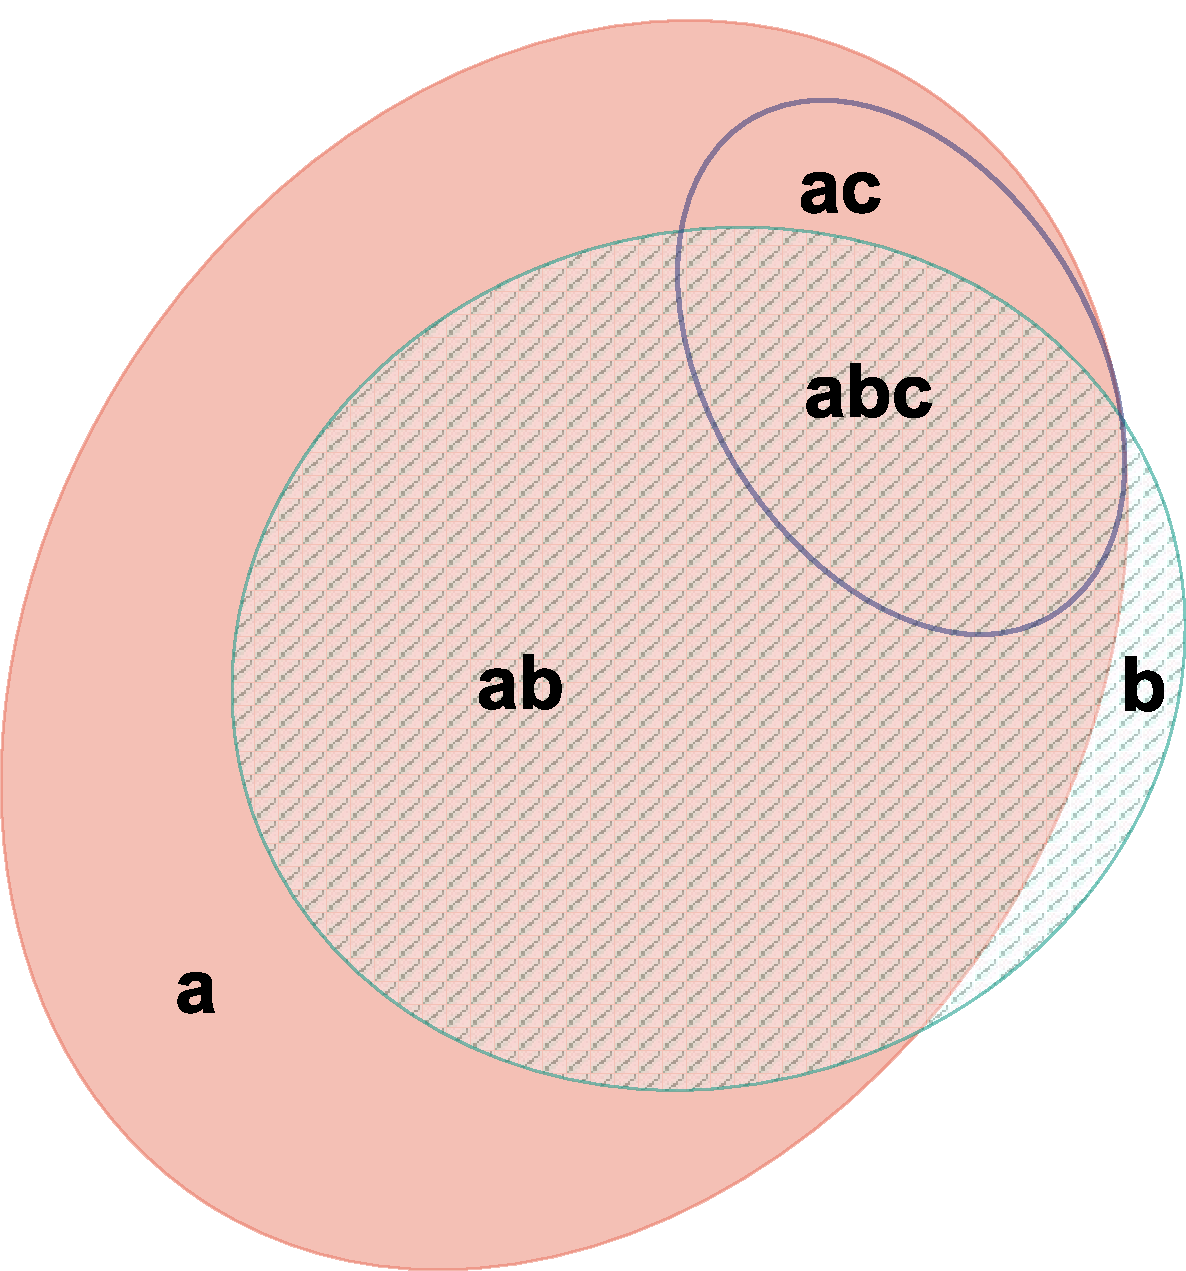
\includegraphics[height=.9\linewidth]{graphics//eulerape-lenz-a}
\subcaption{The diagram from \pkg{eulerAPE}.}
\end{subfigure}
\end{figure}

To conclude the case studies part of this thesis, we look at a diagram
that was featured on website of the author of
\pkg{venn.js}~\citep{Frederickson_2015a}, which used the
\emph{Netflix Prize Dataset}\sidenote{The dataset is no longer available
on this webpage, but can be found at
\url{https://www.kaggle.com/netflix-inc/netflix-prize-data}
for those who are interested.} from which he
\begin{quote}
[...] picked 6 movies, kind of at random -- and then represented them using the
set of users that gave the movie a 5 star rating.
\end{quote}
The movies were Amelie, Pulp Fiction, Miss Congeniality, Armageddon, Rashomon,
and Coyote Ugly. The data only includes pairwise
relationships~(\cref{tab:netflix}).

\begin{table}
\sidecaption{The data from the Netflix Prize dataset
used in \citet{Frederickson_2015a}.\label{tab:netflix}}
\centering
\libertineTabular
\addtolength{\tabcolsep}{-2pt}
\small
\begin{tabular}{r|rrrrrr}
& \rot{Amelie} & \rot{Pulp Fiction} & \rot{Miss Congeniality} & \rot{Armageddon} & \rot{Rashomon} & \rot{Coyote Ugly}\\
\hline
Amelie            & 38,753 &&&&&\\
Pulp Fiction      & 15,197 & 70,153 &&&&\\
Miss Congeniality &  1,829 &  3,854 & 37,837 &&&\\
Armageddon        &  1,218 &  6,593 & 10,536 & 40,345 &&\\
Rashomon          &  2,087 &  2,799 &    132 &    143 & 6,209 &\\
Coyote Ugly       &    610 &  2,206 &  5,965 &  5,699 &    38 & 15,611
\end{tabular}
\end{table}





































